\documentclass[10pt,a4paper]{article}
\usepackage[utf8]{inputenc}
\usepackage[english]{babel}
\usepackage{amsmath}
\usepackage{amsfonts}
\usepackage{amssymb}
\usepackage{graphicx}
%\usepackage{caption}
\usepackage{subcaption}
\usepackage{listings}
\usepackage{color}
\usepackage{hyperref}
\usepackage[
backend=biber,
style=numeric,
sorting=ynt
]{biblatex}
\usepackage{url}
\addbibresource{references.bib}

\definecolor{lightgray}{rgb}{.9,.9,.9}
\definecolor{darkgray}{rgb}{.4,.4,.4}
\definecolor{purple}{rgb}{0.65, 0.12, 0.82}

\lstloadlanguages{Ruby}

\lstdefinelanguage{JavaScript}{
  keywords={typeof, new, true, false, catch, function, return, null, catch, switch, var, if, in, while, do, else, case, break},
  keywordstyle=\color{blue}\bfseries,
  ndkeywords={class, export, boolean, throw, implements, import, this},
  ndkeywordstyle=\color{darkgray}\bfseries,
  identifierstyle=\color{black},
  sensitive=false,
  comment=[l]{//},
  morecomment=[s]{/*}{*/},
  commentstyle=\color{purple}\ttfamily,
  stringstyle=\color{red}\ttfamily,
  morestring=[b]',
  morestring=[b]"
}

\lstset{
   language=JavaScript,
   backgroundcolor=\color{lightgray},
   extendedchars=true,
   basicstyle=\footnotesize\ttfamily,
   showstringspaces=false,
   showspaces=false,
   numbers=left,
   numberstyle=\footnotesize,
   numbersep=9pt,
   tabsize=2,
   breaklines=true,
   showtabs=false,
   captionpos=b,
   escapeinside={(*@}{@*)}
}


\lstnewenvironment{snippet}[1][]
    {\lstset{float=htpb,#1}} 
    {}

\begin{document}
\tableofcontents
\newpage
\section{Introduction}
The goals for this bachelor thesis is to enchance the writers skill in software development. The main theme of the thesis is working with external data through accessing web APIs and use them to create a new service. In this bachelor thesis a web application designed to make a transportation choice simpler is implemented. It is inspired by the pain I was having for choosing if I was going to wait for the bus to get home or if I should walk. The application lets the user find the difference in time between walking, cycling, driving or taking public transport between an origin and a destination. It also provides weather information to make it easier to decide what transportation to choose.
\section{Technical background}
The focus for this bachelor thesis is on obtaining data from different sources and presenting them in a useful way for a user. To achieve this the thesis is based on different technologies. This enables us to experience and compare the different technologies explained in this section.
%During the development of the web application the following technologies and tools were used.

\subsection{Web application framework}
A web application framework is used to develop dynamic websites. 
\begin{figure}[center]
  \centering
  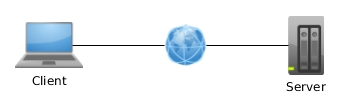
\includegraphics[width=0.5\linewidth]{../webframework/webframe}
  \caption{Client and server in a web application context}
  \label{fig:webapp}
\end{figure}


Hypertext navigation, such as HTML, provides static web pages. These web pages are the same for all users. For a web page to become dynamic it needs to change in response to different contexts or conditions. A dynamic web page can be achieved by client-side scripting (done at the client in figure \ref{fig:arch}) and server-side scripting (done at the server in figure \ref{fig:arch}). Client-side scripting changes the web page by executing code on the client-side. In contrast, server-side scripting executes code on a web server to create a customized response for each users request. The client-side and server-side scripting can be combined or used alone. \cite{webapp}

\subsection{Ruby on Rails}
Ruby on Rails is an open source web application framework that can be used to develop dynamic websites. It is written in the Ruby programming language. \cite{rubyrails}

\subsection{AJAX}
Asynchronous Javascript And XML (AJAX) is a group of web development tools used client side to make asynchronous web applications. With AJAX data can be sent from the client to the server without making changes on the displayed web page. Data can also be retrieved, and the web page can be changed without needing to change the whole web page. Even though the name implies use of XML, it is common to use JSON for data exchange \cite{ajax}.



\subsection{Same-origin policy}
Most web browsers request that data transferred by using AJAX is only transferred between the client and the server on the same domain. It is therefore not possible to transfer data between the client and a server on another domain. This is called same-origin policy, and is used to increase security. In figure \ref{fig:sameorigin} it is illustrated how the policy works. The client can send AJAX to the web server that has the same domain as the client is visiting. If the client try to send regular AJAX to another server, the data will not come through and get lost. \cite{sameorigin}



\begin{figure}
\centering
\begin{subfigure}{0.45\textwidth}
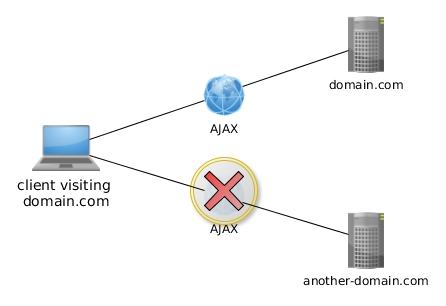
\includegraphics[width=\textwidth]{../ajax/ajax}
\caption{Same-origin policy}
\label{fig:sameorigin}
\end{subfigure}
\begin{subfigure}{0.45\textwidth}
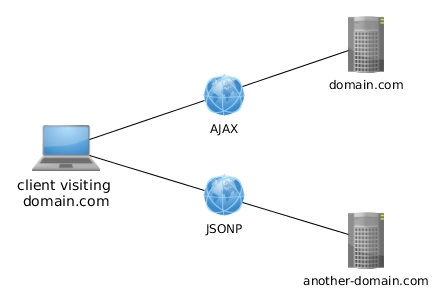
\includegraphics[width=\textwidth]{../jsonp/jsonp}
\caption{JSONP}
\label{fig:jsonp}
\end{subfigure}
\end{figure}

\subsection{JSONP}

JSONP is a way of sending and receiving data from the client web browser to another domain, thus avoiding the same origin policy. It works by exchanging data by using $\langle$ script $\rangle$ tags. This tag is not enforced by the same origin policy, as shown in figure \ref{fig:jsonp}.\cite{jsonp}


\subsection{Application Programming Interface (API)}
Application Programming Interface is a set of routines, protocols and tools for building software applications. There are a wide range of APIs. For example, in a programming language a library provides functions for the programmer to use. The library's API explains how to use these functions for the programmer, so that the programmer don't need to look at the implementation of the functions. \cite{api}
\subsection{Mashup}
A mashup is a web page that uses content from more than one source to create a single new service. An  example is taking data from several web services and displaying them on a web page. \cite{mashup}
\subsection{Web API}
A web API defines the interface through which interactions happen between an enterprise and application that use its assets. For the application to get these assets from the enterprise it has to send a HTTP request over a network. This request has to contain data that uses the web API for the enterprise to understand what asset the application want. When the enterprise has received the HTTP request, it sends back a HTTP response. This HTTP response is usually in XML or JSON format. \cite{webapi}

\subsection{RESTful API}
\label{sec:restful-api}
REpresentational State Transfer (REST) is, among other things, a client-server architecture that uses the HTTP protocol for communication. A RESTful API is an API that uses this client-server architecture for communication. Each URL on the server represents a resource, for example: news.com/item/3. In this example the resource ``item 3'' is accessible by visiting this url. The different HTTP methods (GET, POST, PUT, DELETE) are used for operiting on the resources. Some, mostly older, web APIs are based on SOAP, which is a more complicated to use.\cite{rest}

\subsection{YQL}
Yahoo! Query Language is designed to retrieve and manipulate data from APIs. This allows users to get data from an API and remove information that is not needed. \cite{yql}

\subsection{Ruter.no API}
\label{sec:ruter.no-api}
Ruter is the public transport authority for Oslo and Akershus\cite{ruterinfo}. With their API they provide access to real time data for all public transportation in Oslo and Akershus.

\subsection{met.no API}
\label{sec:met.no-api-1}
Norwegian Meterological Institute (MET norway) provides weather forecasts for Norway. They provide free access to the weather data through their API. \cite{metnoinfo}

\subsection{Google Maps javascript API}
\label{sec:google-maps-javascr-1}
Google Maps is a service from Google. It provides, among other things, a route planning tool. This tool can be accessed by using the Google Maps javascript API. The API is free for commercial use, with some restrictions. \cite{gmapsinfo}

\subsection{Heroku}
\label{sec:heroku}
Heroku is a Platform as a service (PaaS)\cite{herokuinfo}. This means it provide a platform that allows customers to develop, run and manage web applications without the complexity that is normally associated with launching the application online\cite{paas}.

\subsection{Firebug}
Firebug is a web browser extension for Firefox. It makes it possible to, among other things, track the time of AJAX and JSON. \cite{firebug}

\subsection{Traceroute}
Traceroute is a computer network tool for displaying the path of packets across an IP network. \cite{traceroute}
\section{Design}
In this section the method of getting the data is explained. I gave my application the name ``Kostr'', which is the norse translation of choice.

\subsection{Obtaining data}
\label{sec:architecture}



\begin{figure}
\centering
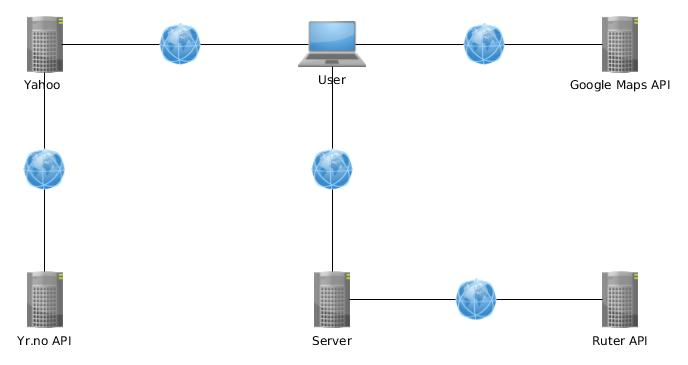
\includegraphics[width=\textwidth]{../arch/arch}
\caption{Architecture}
\label{fig:arch}
\end{figure}

Below is a list of all the servers that the application uses to create the mashup service. All of the servers in the list are found in figure \ref{fig:arch}.

\begin{itemize}
\item YQL server. Used to access the met.no server.\cite{yql}
\item met.no server. Used to get weather data.\cite{metno}
\item Google Maps server. Used to get walking, cycling and driving data.\cite{gmaps}
\item Ruter.no server. Used to get public transport data.\cite{ruter}
\item Kostr server. Used to access the Ruter.no server and to host the Kostr website.
\end{itemize}

The four first servers in the list are external servers that is not maintained by the application. The fifth server is maintained by the application. All the external servers are accessed by using a web API defined by the companies in control of the servers. All of the servers are accessed by using either AJAX or JSONP.

\subsubsection{Accessing the met.no server}
\label{sec:access-weath-api}
\begin{figure}
\centering
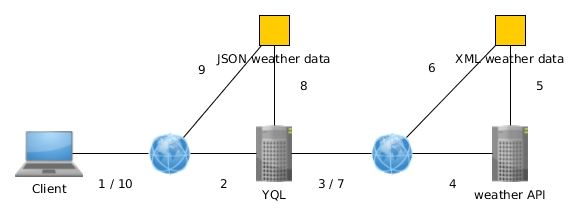
\includegraphics[width=\textwidth]{../weather/access}

\caption{Weather API}
\label{fig:weather}
\end{figure}

To get weather data the application uses javascript that runs on the client side. The javascript uses JSONP to request data from YQL. In figure \ref{fig:weather} the steps taken to get the data is illustrated. It provides YQL with information that is needed to get the correct data from the met.no server (steps 1 and 2). YQL requests the information from the weather API (steps 3 and 4). The weather API finds the weather data and sends it to YQL(steps 5, 6 and 7). YQL extract the data from the XML document that YQL required and sends this data in JSONP format to the client (steps 8, 9 and 10).

\subsubsection{Accessing the Ruter.no server}
\label{sec:access-publ-transp}
\begin{figure}
\centering
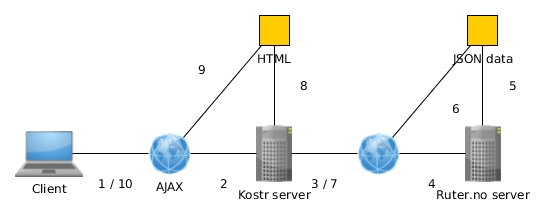
\includegraphics[width=\textwidth]{../ruter/access}
\caption{Public transport API}
\label{fig:public}
\end{figure}
To get the public transport information the client need to access the Ruter.no server. The steps required to get the information is shown in figure \ref{fig:public}. It sends the origin and destination location to the Kostr server by using AJAX (steps 1 and 2). The server converts the source and destination to UTM coordinates and sends an HTTP request to Ruter API (steps 3 and 4). The Ruter server finds several possible routes and sends an HTTP response back to the server (step 5, 6 and 7). The server chooses the first route and extracts the information needed and sends it using AJAX to the client (steps 8, 9 and 10).

\subsubsection{Accessing the Google Maps server}
\label{sec:access-google-maps}
\begin{figure}
\centering
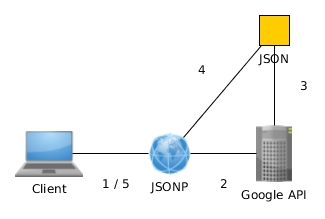
\includegraphics[width=0.6\textwidth]{../google/access}
\caption{Google Maps API}
\label{fig:google}
\end{figure}
To get information about walking, cycling and driving the javascript on client side uses the Google Maps javascript API. The steps required to get the information is shown in figure \ref{fig:google}. This API also uses JSONP for exchange of data. The client uses the source and destination as arguments in the javascript call (steps 1 and 2). The Google API server try to find one or several routes that go between the source and the destination requested by the client. It then sends the route(s) in JSON format to the client (steps 3, 4 and 5).

% End systems are connected together by a network of communication links and packet switches. 
% End systems attached to the Internet provide an Application Programming Interface that specifies how a program running on one end system asks the Internet infrastructure to deliver data to a specific destination program running on another end system. 

% An optical fiber is a thin, flexible medium that conducts pulses of light, with each pulse representing a bit. 

\subsection{User interface}
\label{sec:user_inter}

The user interface consist of one single page. This is accomplished by exchanging all data using AJAX and JSONP routines. Figure \ref{fig:ux_empty} shows the page the client sees when visiting the website with the application. The website has a form that lets the client enter a origin and destination location. It also lets the client restrict which type of transportation it would like to get information about. The origin and destination form fields implements an autocomplete feature that lets the user easierly find the address they want to travel from and to, as shown in figure \ref{fig:ux_autocomplete}. \\
\begin{figure}[h]
  \centering
  \begin{subfigure}{0.4\textwidth}
    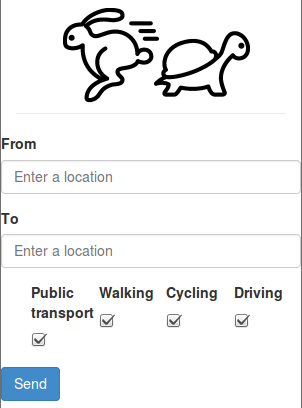
\includegraphics[width=\textwidth]{../ux/empty}
    \caption{Empty forms}
    \label{fig:ux_empty}    
  \end{subfigure}
\hfill %\qquad
  \begin{subfigure}{0.4\textwidth}
    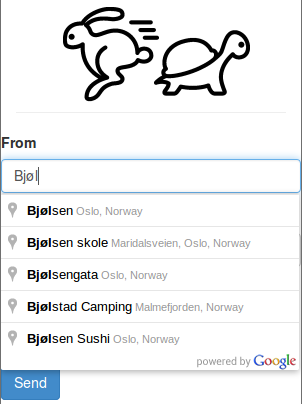
\includegraphics[width=\textwidth]{../ux/autocomplete}
    \caption{Autocomplete}
\label{fig:ux_autocomplete}
  \end{subfigure}
  \caption{User interface}
  \label{fig:ux_first}
\end{figure}
In figure \ref{fig:ux_filled} the forms are filled out by the user. When the user press the send button the data is sent to the different servers mentioned in section \ref{sec:architecture}. The application then receives data from the servers and display the output. An example is displayed in figure \ref{fig:ux_result}. The output contains an image representing the weather at the origin place, shown on top of the figure. It also contains information about each of the selected transportations. To the left of the walking, cycling and driving information is a link the client can click to get the directions displayed on http://maps.google.com.
\begin{figure}[h]
  \centering
  \begin{subfigure}{0.4\textwidth}
    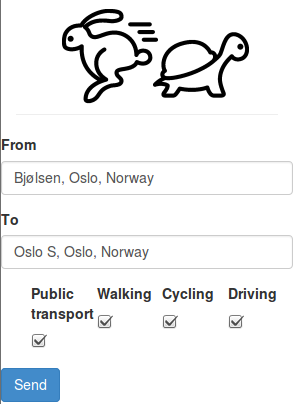
\includegraphics[width=\textwidth]{../ux/filled}
    \caption{Filled forms}
    \label{fig:ux_filled}
  \end{subfigure}
\hfill
\begin{subfigure}{0.4\textwidth}
  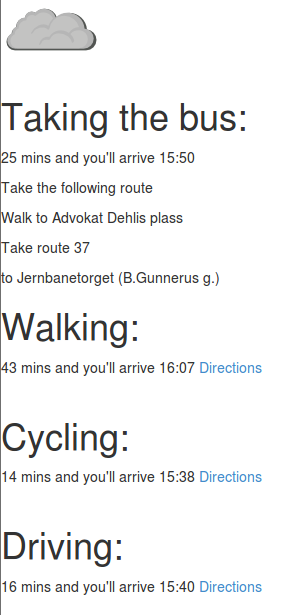
\includegraphics[width=\textwidth]{../ux/result}
  \caption{Search result}
  \label{fig:ux_result}
\end{subfigure}
  \caption{User interface}
  \label{fig:ux_last}
\end{figure}

\section{Implementation}

\subsection{Exchanging data from the web application ...}
\label{sec:sending-data-from}
In this section the implementation of how data is exchanged between the web applications to the different servers will be explained. The explanation will describe what happens from the client click the ``send'' button until the results are displayed. In listing \ref{lst:event} is an overview of what happens when the 'send' button is pressed. When the client click ``send'' the a javascript event handler (line \ref{event_handler}) is executed on the client side. The event handler executes the functions that perform the exchange of data between the servers. (All listings in this section does not give the complete implementation and is simplified to give the reader a better understanding.)

\begin{lstlisting}[caption=Event handler, label=lst:event]
jQuery.('send').click(function () { (*@\label{event_handler}@*)
  ajaxToWebServer(origin, destination);
  getGoogleRoutes(origin, destination);
  getWeatherInfo(origin);
});
  
\end{lstlisting}
\subsubsection{to the Google Maps server}
\label{sec:google-maps-javascr}
When the page is loaded at the client it includes a large javascript file that contain the Google Maps javascript API. This file contains methods for using the API.
When the client click ``send'' the a javascript event handler is executed on the client side. The event handler executes the function that creates a request and sends it to the Google Maps API server by using the function at line \ref{googlecall} in listing \ref{lst:google}. When the response is received, the callback function is  executed. It calculates the time for when the client is to arrive and then displays the information to the client.

\begin{lstlisting}[caption=Using the Google Maps javascript API, label=lst:google]

function callback(response) {
  var trip = response.trip;
  var time = calculateTimeForTrip(trip);
  displayTripAndTime(trip, time);
}

function getGoogleRoutes(origin, destination) {
  request = google.createRequest(origin, destination);
  setOptionsForRequest(request);
  google.getResponseAndCallCallback(request, callback); (*@\label{googlecall}@*)
}
  
\end{lstlisting}

\subsubsection{to the met.no server}
\label{sec:met.no-api}
The 
\begin{lstlisting}[caption=Using YQL API and met.no API to access met.no server, label=lst:metno]
function callback(data) {
  var weather = parseYqlResult(data);
  displayWeather(weather);
}

function getWeatherInfo(origin) {
  var locationOfOrigin = getLocationOfOrigin(origin);
  var metRestUrl = "http://api.met.no/weatherapi/locationforecast/1.9/?";
  var baseUrl = "http://query.yahooapis.com/v1/public/yql?q=";
  var query = "select * from xml where url=";
  
  var url = baseUrl + query + metRestUrl + locationOfOrigin;
  jQuery.getJSON(url, callback);
}

\end{lstlisting}
\subsection{Using the Ruter.no API}
\label{sec:using-ruter.no-api}


\begin{lstlisting}[caption=Using Ruter.no API to access Ruter.no server, label=lst:ruter, language=Ruby]
class Ruter
	def self.getRoute(query)
		return get('/travel/gettravels/', query: query)
	end
end

class TripsController < ApplicationController

    def create(parameters)
      utmLocations = convertToUTM(parameters)
      query = makeRuterQuery(utmLocations)
      trip = Ruter.getRoute(query)
      trip.metadata = calculateMetadata(trip)
      trip.save #save to database
      
      sendWithAjaxToClient(tripToHtml(trip))
    end
end
\end{lstlisting}



\section{Discussion}

\subsection{Location of web API servers}
By using traceroute it is possible to find the IP addresses of the servers that the web APIs access. By using a geolocation software it is possible to find the location of these IP addresses. In figure \ref{fig:traceroute_heroku} the server is hosted by Heroku. In figure \ref{fig:traceroute_localhost} the web server is hosted on the client computer. In the list below is the explanation of each letter on the map:
\begin{itemize}
\item A is the client and the Kostr server when run locally.
\item B is the Google Maps server.
\item C is the YQL server.
\item D is Kostr server when run remotely on Heroku.
\item E is the Ruter server and the met.no server.
\end{itemize}

\begin{figure}
\centering
\begin{subfigure}{\textwidth}
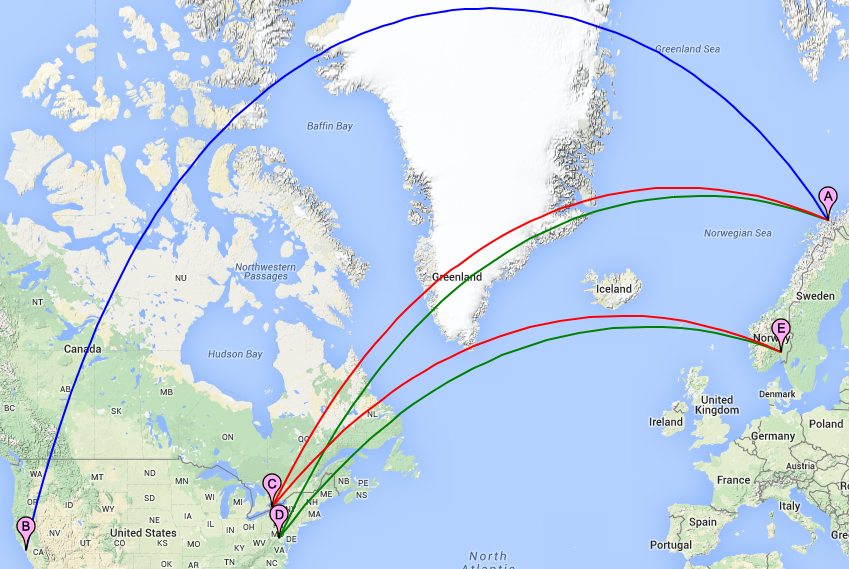
\includegraphics[width=\textwidth]{../traceroute/heroku_markers}
\caption{Web server run remotely on Heroku.}
\label{fig:traceroute_heroku}
\end{subfigure}


\begin{subfigure}{\textwidth}
\centering
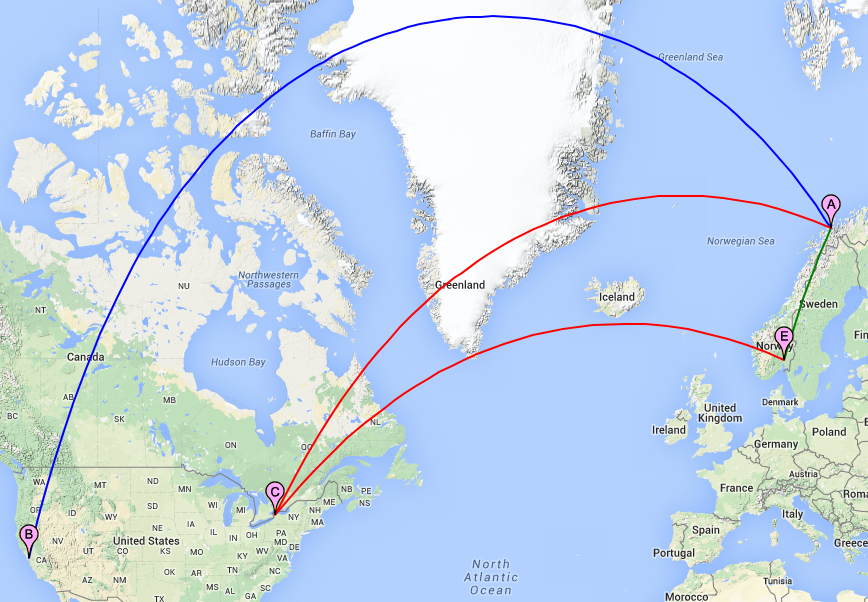
\includegraphics[width=\textwidth]{../traceroute/localhost_markers}
\caption{Web server run locally on clients computer }
\label{fig:traceroute_localhost}
\end{subfigure}
\caption{Each letter represents a location found by traceroute. A is the client and the web server when run locally. B is the Google Maps API server. C is the YQL server. D is heroku server. E is the Ruter API server and the YR API server.}
\label{fig:traceroute}
\end{figure}

\subsection{Common access routes}
Both architectures access the Google Maps javascript API, YQL API and weather API in the same manner. 

\subsubsection{Accessing the met.no API server}
In figure \ref{fig:traceroute} we see that when accessing the met.no API the HTTP request is first sent to the YQL API server (C in figure \ref{fig:traceroute} a and b). This is the same route as shown in figure \ref{fig:weather} step 1 and 2. The YQL server then sends an HTTP request to the met.no API server(E in figure \ref{fig:traceroute} a and b), as shown in figure \ref{fig:weather} step 3 and 4. The met.no API server then uses the information from the request and finds the weather data and sends it to the YQL server in XML server, step 5, 6 and 7 in figure \ref{fig:weather}. The YQL server extracts the needed information from the XML data, converts it to JSON and sends it back in an HTTP response to the client, step 8, 9 and 10 in figure \ref{fig:weather}.

\subsubsection{Accessing the Google Maps API server}
In figure \ref{fig:traceroute} the Google Maps API server is accessed by sending an HTTP request from the user (marker A) to the API server (marker B). This is show as step 1 and 2 in figure \ref{fig:google}. The API server finds route suggestions and send the data back in a HTTP response to the client. This is shown as step 3, 4 and 5 in figure \ref{fig:google}.

\subsection{Web server access routes}
\label{sec:web-server-access}
When the web server is run locally, the Ruter API server access route is shorter. As seen in figure \ref{fig:public}, the data sent in steps 1, 2, 9 and 10 travels a shorter distance. 
\subsubsection{Accessing the Ruter.no API server}
\paragraph{Remote web server}
In figure \ref{fig:traceroute_heroku} the client sends an HTTP request to the Heroku server at marker D. The Heroku server then sends an HTTP request to the Ruter API server at marker E. The response HTTP is then sent to the Heroku server. The heroku server processes the data and sends an HTTP response to the client.
\paragraph{Local web server}
In figure \ref{fig:traceroute_localhost} the client sends an HTTP request to the local server, which is also at marker A. The local server sends an HTTP request to the Ruter.no API server. The response HTTP is then sent to the local server. The local server processes the data and sends an HTTP response to the client.




\subsection{Performance}
\label{sec:performance}
By using Firebug it is possible to see how long the access time is for each of the APIs. The times vary between each HTTP request because of different congestion on the network and different server load and/or performance on the API servers. The results are a result of making 10 HTTP requests and take the average of the times. 
\begin{figure}
\centering
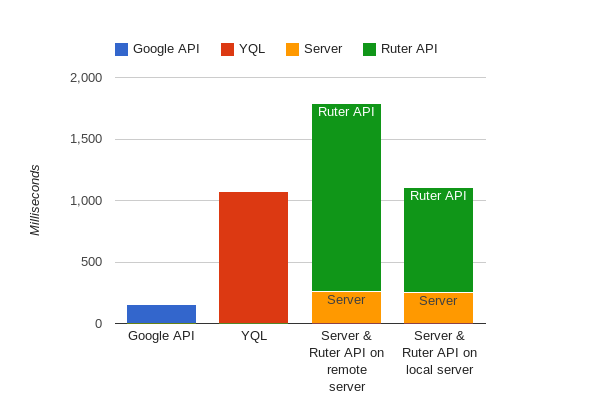
\includegraphics[width=\textwidth]{../apitimes/apitider}
\caption{API access times}
\label{fig:time}
\end{figure}

\subsubsection{Common access route performance}
In figure \ref{fig:time} is the access time for the application when the server is run remotelyand when run locally.

\paragraph{Google API server access time} 
In figure \ref{fig:google} and figure \ref{fig:traceroute} the access to the Google API access one less server than the rest of the API requests. This could give a sign that the access time should be shorter than for the other API accesses. In figure \ref{fig:time} we see that the access time for the Google API server is under 200 milliseconds. Even though the distance between the client and the Google API server is longer than the client to the other intermediary servers, the time saved by only accessing one server instead of two gives a time benefit.

\paragraph{met.no API access time} 
In figure \ref{fig:weather} and figure \ref{fig:traceroute} it shows that the access to the met.no API server requires an intermedia server access to the YQL API server. In figure \ref{fig:time} it shows that the access time is 1000. This is more than 5 times greater than the access time to the Google API server. One of the reasons is that the data retrieval requires two server accesses. Another reason can be that either or both of the servers hosting the APIs have a slower performance than Googles.

\subsubsection{Web server access routes performance}
\paragraph{Ruter.no API access time}
In figure \ref{fig:public} and figure \ref{fig:traceroute} is shown that the access to the Ruter.no API server requires intermedia server access on the web applications server. The placement of the web application server is different as mentioned in section \ref{sec:web-server-access}. This resulted in difference in access time for accessing the Ruter.no API server, as shown in figure \ref{fig:time}. When the web application server is hosted remotely on heroku the access time for the Ruter.no API is 1800 milliseconds. When it is hosted locally the access time for the Ruter.no API is 1100. Thus there is a difference in 700 milliseconds. The access time for the Ruter.no API server is divided into two sections. The server access time is 250 milliseconds. It is the same for both the server hosted locally and remotely. The reason for this can be that the server hosted locally uses more time to process the result from the Ruter.no API. The Ruter.no API access time has a difference of 700 milliseconds. The access time for the Ruter API server from the web application server was 1550 milliseconds when the server is hosted remotely, while it was 850 milliseconds when it is hosted locally. One of the reasons is that the location of the Ruter.no API server is faster to access from the clients location. 

%Some of the difference can be explained by the reasons mentioned in section \ref{sec:performance}. 


\section{Conclusion}

\newpage
\printbibliography
\end{document}
%%% Local Variables:
%%% mode: latex
%%% TeX-master: t
%%% End:

